











	
	Zastosowanie deep learningu do generowania w ostatnim czasie stało się bardzo popularne. Szybki rozwój frameworków takich jak Tensorflow czy Keras pozwala na sprawne budowanie modeli, a wykorzystanie chmur obliczeniowych zwalnia programistę z używania własnego sprzętu bądź też kupowania drogich procesorów GPU. Poniższa grafika obrazuje liczbę publikacji wydanych na przestrzeni ostatnich trzydziestu lat poświęconych generowaniu muzyki z wykorzystaniem deep learningu.
	
	\begin{figure}[H]
		\centering
		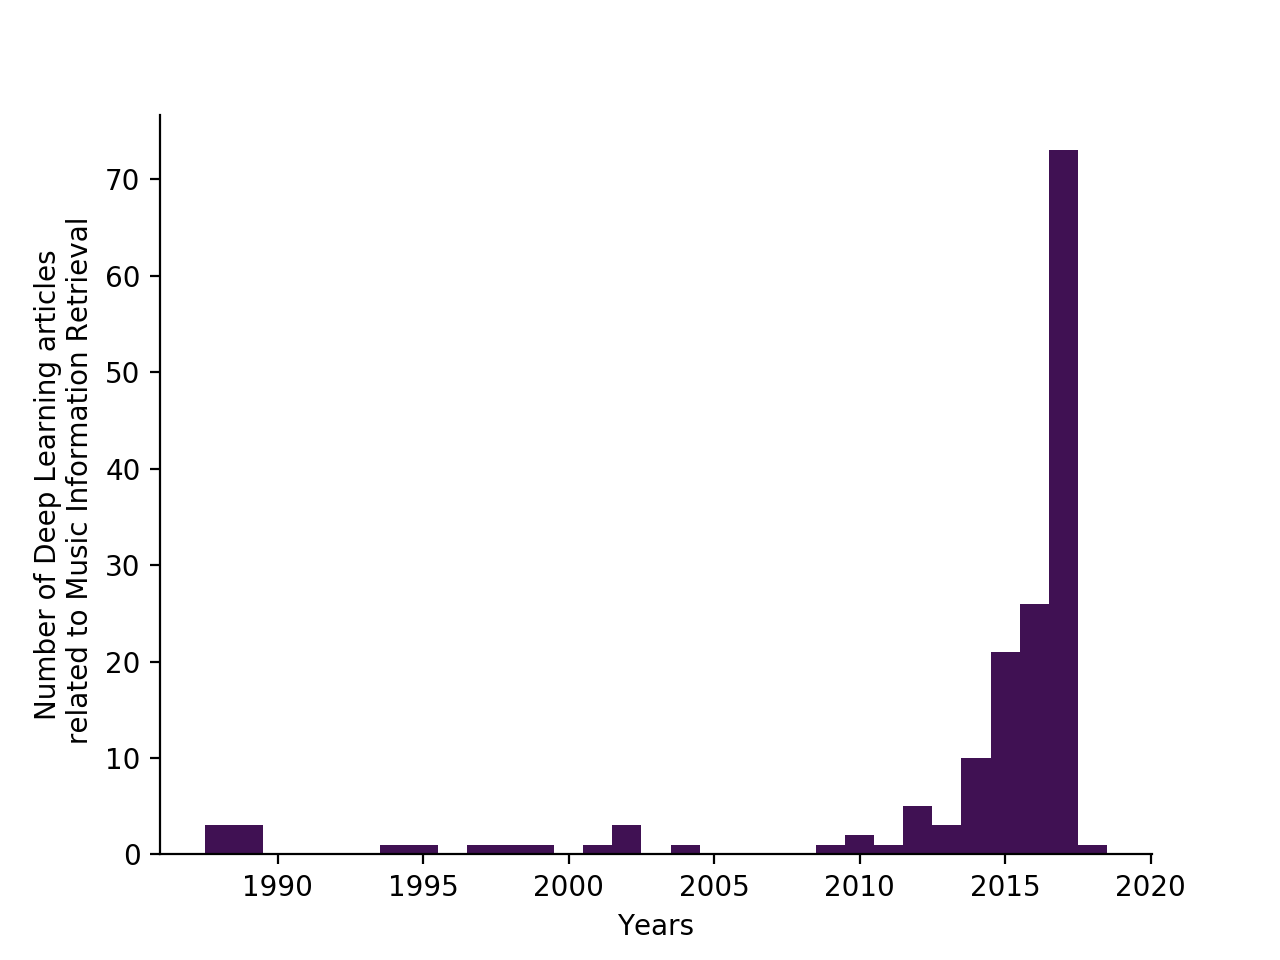
\includegraphics[width=0.7\linewidth]{xxxxxxxxxx}
		\caption{Znaczący wzrost publikacji zanotowany w ostatnich latach $\pagenote{https://github.com/ybayle/awesome-deep-learning-music/blob/master/dl4m.bib}$}
		\label{fig:xxxxxxxxxx}
	\end{figure}
	
	Obecnie na rynku można wyróżnić sześć dużych projektów związanych z automatycznym generowaniem muzyki:
	
 $\textbf{Magenta}$ - jest to projekt na licencji open source stworzony przez Google. Jak sami autorzy piszą Magenta jest projektem badawczym, który bada rolę uczenia maszynowego w procesie tworzenia sztuki i muzyki. Wiąże się to z ciągłym poszukiwaniem nowych algorytmów deeplearningu. Projekt stanowi również bogate zródło inspiracji dla muzyków i artystów, ponieważ mogą oni wzbogacić swoje procesy za pomocą modeli deep learningu. Przykładem może być tutaj projekt Duet AI$\pagenote{https://experiments.withgoogle.com/ai-duet}$. Magenta powstała na skutek prac inżynierów i badaczy z Google Brain$\pagenote{https://ai.google/research/teams/brain}$. Cały projekt bazuje na frameworku Tensorflow, jego źródła zostały upublicznione w czerwcu 2016. Aktualnie Magenta implementuje standardową sieć rekurencyjną oraz dwie sieci LSTM. W użyciu biblioteka sprawuje się bardzo dobrze, ponieważ posiada modele wytrenowane na tysiącach plików midi. Istnieje możliwość stworzenia własnego modelu na podstawie własnych plików midi. Niestety projekt nie posiada szczegółowej dokumentacji. Magenta może generować tylko jeden strumień nut. Nie ma możliwości połączenia kliku modeli np. pianino z perkusją czy gitarą. Trwają prace aby stworzyć model, który będzie wstanie przetwarzać muzykę polifoniczną oraz tworzyć harmonię. 
  
 $\textbf{DeepJazz}$ - jest efektem pracy Ji-Sung Kima podczas 36 godzinnego hackathonu. Model zawiera dwie warstwy sieci LSTM, które uczą się na podstawie sekwencji nut z plików midi. Projekt cieszy się bardzo dużą popularnością mimo tego, że nie jest tak skomplikowany jak Magenta. Model jest wstanie wygenerować nowy utwór na podstawie tylko jednego pliku midi. Projekt został stworzony wykorzystując biblioteki Keras, Theano oraz Tensorflow.
 
 $\textbf{BachBot}$ - projekt badawczy stworzony przez FeynmanaLianga na uniwersytecie w Cambridge. BachBot również wykorzystuje sieci LSTM. Danymi treningowymi są chorały Bacha. Celem modelu jest generowanie i harmonizowanie chorałów. Badania autora wykazały, że ludziom trudno jest odróżnić wygenerowany chorał od prawdziwego dzieła Bacha. Model wyróżnia się tym na tle innych, że może maksymalnie obsłużyć aż cztery głosy.
 
 $\textbf{FlowMachines}$ - projekt badawczy, który został sfinansowany przez Europejską radę ds. Badań Naukowych w ramach 70 programu ramowego UE. Badania zostały zapoczątkowane przez francuskiego naukowca Francoisa Pachet w Sony Computer Science Laboratories (Sony SCL Paris) oraz Uniwersytet Piotra i Marii Curie (UPMC). Celem projektu FlowMachines jest badanie i rozwijanie systemów sztucznej inteligencji zdolnych do generowania muzyki samodzielnie lub we współpracy z ludźmi. W roku 2017 dzięki FlowMachines udało się wygenerować pełny utwór muzyczny gatunku pop$\pagenote{https://www.youtube.com/watch?v=LSHZ\_b05W7o}$. 
 
 $\textbf{WaveNet}$ - projekt badawczy naukowców z DeepMind. WaveNet bazuje na Konwolucyjnych Sieciach Neuronowych, ta technika bardzo dobrze sprawdza się w klasyfikacji i generowaniu obrazów. Najbardziej obiecującym celem projektu jest poprawa zastosowań zamiany testu na mowę poprzez wygenerowanie bardziej naturalnego przepływu wokalu. WaveNet pobiera surowy sygnał audio i syntezuje próbkę wyjściową na podstawie próbki wejściowej. Projekt nie jest oparty o wolny kod źródłowy, ale doczekał się implementacji przez społeczność. Dzięki temu, że sieć używa surowego pliku audio jako wejścia, może generować dowolny instrument. $\pagenote{https://github.com/ibab/tensorflow-wavenet}$ Wykorzystane algorytmy w projekcie są bardzo kosztowne obliczeniowa. Potrzeba kliku minut treningu po to aby wygenerować sekundę dźwięku. Jeden z badaczy pracujący dla Google Sageev Oore z projektu Magenta opisał na swoim blogu jakie wnioski może wyciągnąć kompozytor z wyjścia sieci WaveNet$\pagenote{https://magenta.tensorflow.org/2016/09/23/learning-music-from-learned-music}$.
 
 $\textbf{GRUV}$ - kolejny projekt badawczy z Uniwersytetu Stanforda. GRUV podobnie jak WaveNet próbuje wykorzystać surowy sygnał audio jako dane wejściowe. W przeciwieństwie do WaveNet GRUV wykorzystuje sieci LSTM zamiast CNN. Projekt został opublikowany w 2015 roku$\pagenote{https://github.com/MattVitelli/GRUV}$. Naukowcy z Uniwersytetu Stanforda byli jednymi z pierwszych, którzy pokazali w jaki sposób generować nuty za pomocą sieci LSTM wykorzystując surowe pliki audio jako dane wejściowe. 
 
 
 Moc i wszechstronność rekurencyjnych sieci neuronowych nie była powszechnie znana aż to maja 2015 kiedy to amerykański naukowiec Andrej Karpathy opublikował artykuł \textit{The Unreasonable Effectiveness of Recurrent Neural Networks}. Autor pokazał w nim, że stosunkowo prosty model językowy, który nazwał Char-RNN może generować zgodnie ze stylem i wyglądem tekst Szekspirowski czy kod języka C++. Artykuł Andreja pojawił się w czasie kiedy zainteresowanie rekurencyjnymi sieciami neuronowymi było bardzo duże. Wiele osób zastosowało model zaprezentowany przez Andreja Karpathego do generowania muzyki z notacji ABC. 
 
 
 
 \subsection{Reprezentacja danych}
 
 Aplikacje służące do generowania muzyki można podzielić na dwie kategorie ze względu na rodzaj danych wejściowych. Muzyka jest dostępna w różnych cyfrowych formatach. Począwszy od surowego audio (WAV) do formatów, które pozwalają na zapis semantyki utworu muzycznego - są to formaty takie jak MIDI czy notacja ABC. Aby zdecydować, który format danych jest właściwy należy najpierw postawić pytanie o to w jaki sposób sieć neuronowa będzie pracować i jaka będzie jej architektura. 
 
 Surowy format audio jest bardzo bogatą reprezentacją muzyki, ponieważ potrafi przechować niemal każdy szczegół utworu muzycznego w zależności od formatu i jakości dźwięku. Sygnały audio zawierają barwę instrumentu na podstawie charakterystyki spektrum. Aby wyodrębnić poszczególne nuty z surowego pliku audio konieczne jest zastosowanie transformaty Fouriera. Ze względu na to zastosowanie plików audio jako wejście do sieci neuronowej jest dość złożonym przedsięwzięciem. 
 
 W pracy praktycznej został wykorzystany format MIDI ze względu na możliwość bezpośredniego wyodrębnienia nut z pliku.

\begin{figure}[H]
	\centering
	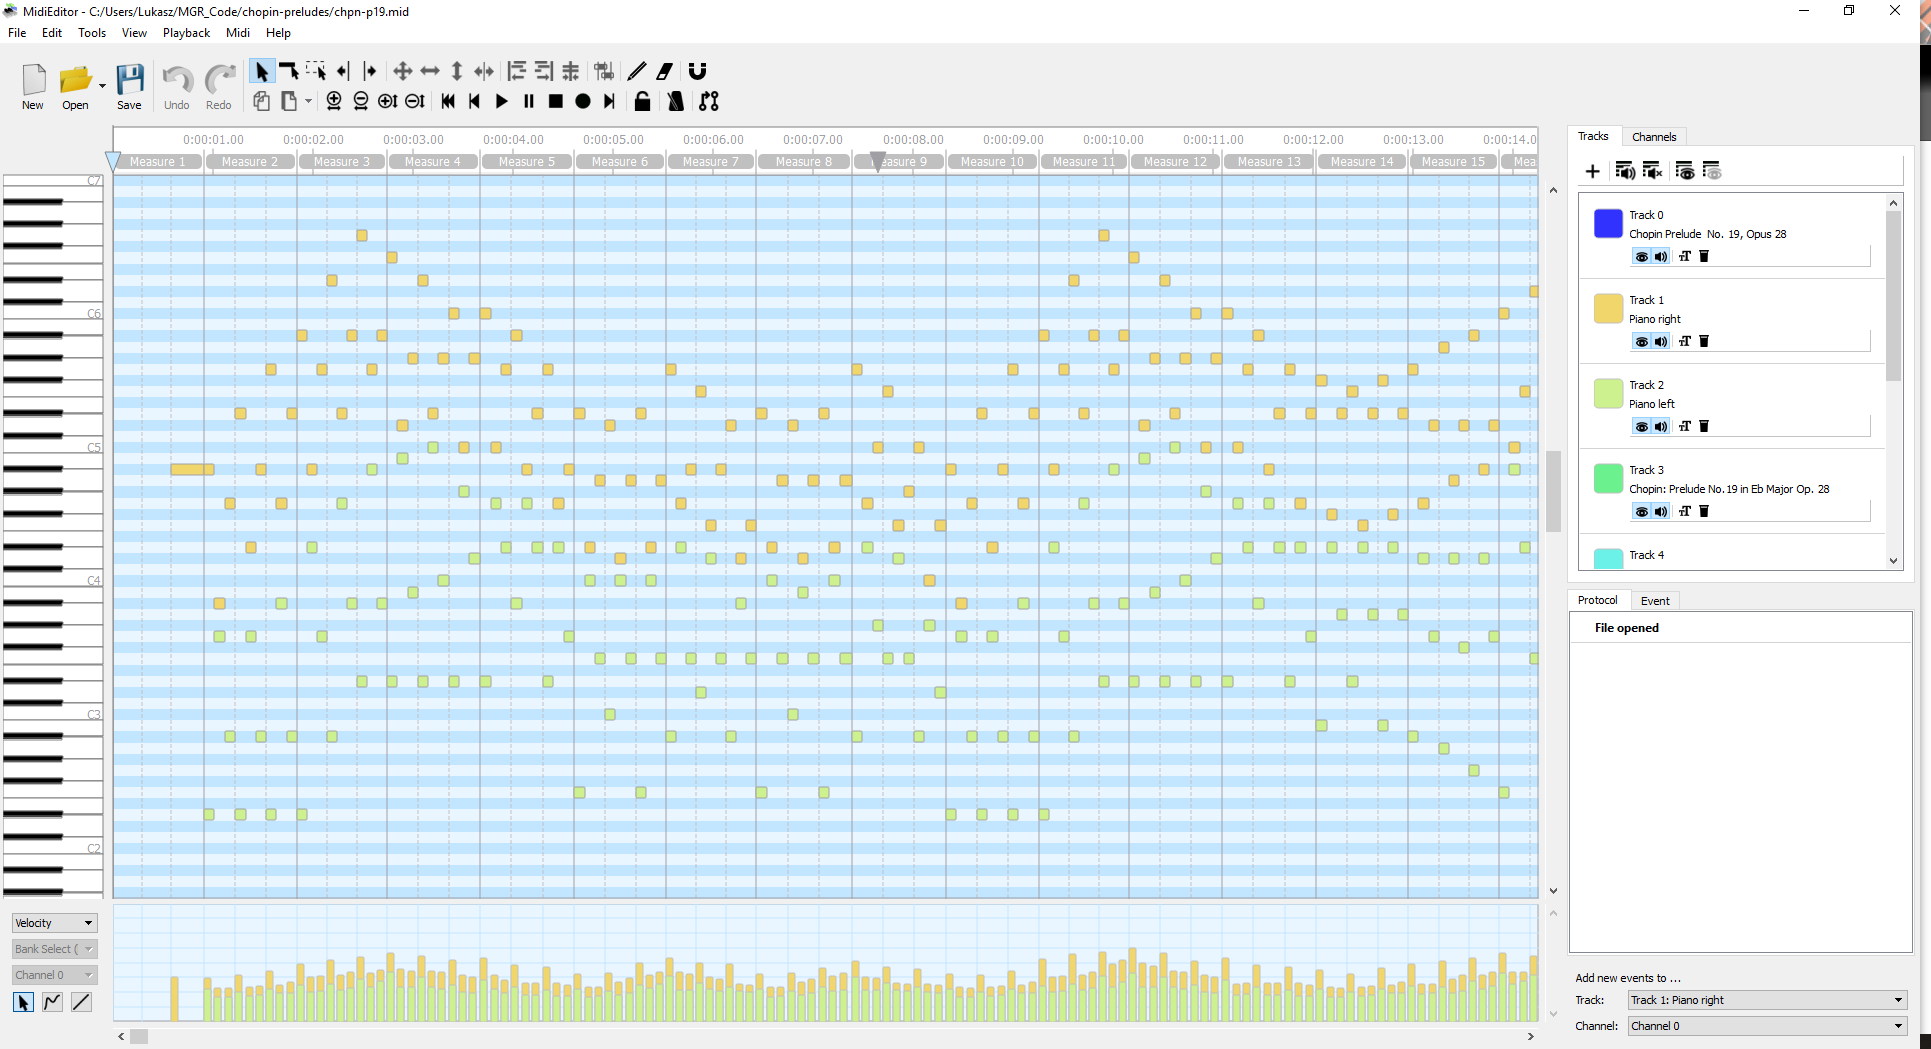
\includegraphics[width=0.8\linewidth]{piano_roll}
	\caption{Reprezentacja pliku midi w programie MidiEditor}
	\label{fig:pianoroll}
\end{figure}

Inspiracją do stworzenia modelu były rozwiązania zastosowane w modelach przeznaczonych do generowania tekstu. W modelowaniu językowym danymi wejściowymi zazwyczaj jest sekwencja słów, a wynik to sekwencja przewidywanych słów. Dana jest długość sekwencji $n$. Sieć ma za zadanie nauczyć się litery, która występuje bezpośrednio po sekwencji długości $n$. Poniżej przykład na podstawie fragmentu Pana Tadeusza.

 
\lstinputlisting[caption=Pan Tadeusz, style=customc]{pan.txt}

Ustalmy długość sekwencji $n=10$, wówczas ciągi odpowiadające danej literze będą wyglądały następująco:

\lstinputlisting[caption=Sekwencje wszystkich możliwych ciągów, style=customc]{panseq.txt}

Jako dane wejściowe do sieci zostaną wykorzystane 24 preludia Fryderyka Chopina w formacie midi. Pierwszy etap polega na przygotowaniu danych. Polega to na stworzeniu tablicy, która będzie zawierała wszystkie nuty z wszystkich 24 dzieł. Docelowo tablica składa się 14098 nut. Początkowy wycinek z tablicy: $\textit{['C2', 'G3', 'G2', 'C4', 'E3', 'G4', 'E4', 'C4', 'A4', 'A3', 'B1', 'G3', 'G2', 'D4', 'F3', 'G4', 'F4', 'D4', 'A4', 'A3']}$ odpowiada pierwszemu preludium z opusu 28. Tablica przechowuje tylko wysokość danej nuty, inne cechy utworu muzycznego nie są wykorzystywane.

\begin{figure}[H]
	\centering
	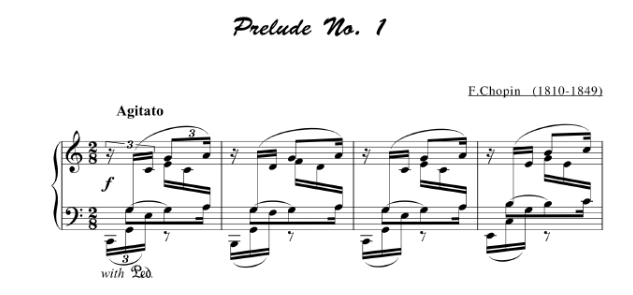
\includegraphics[width=0.7\linewidth]{prelude_no_1}
	\caption{Początkowy fragment preludium}
	\label{fig:preludeno1}
\end{figure}

Liczba wszystkich unikalnych nut wynosi 246, liczba jest tak duża ponieważ uwzględniono w niej wszystkie unikalne kombinacje akordów. Kolejnym krokiem jest stworzenie słownika, który przyporządkuje daną nutę lub akord kolejnej liczbie naturalnej. Rozmiar słownika powinien wynosić tyle ile jest unikalnych nut i akordów czyli 246.

Następnie musimy stworzyć sekwencje wejściowe dla sieci i ich odpowiednich wyjść. Wyjście dla każdej sekwencji wejściowej będzie pierwszą nutą lub akordem, która pojawia się po sekwencji nut w sekwencji wejściowej na naszej liście nut.

\lstinputlisting[caption=Sekwencje wejściowe i odpowiadające im nuty, style=customc]{noteseq.txt}

Do przewidywania prawdopodobieństwa użycie średniego błędu kwadratowego (RMSE) jako funkcji kosztu nie jest właściwe. Jako funkcja kosztu zostanie wykorzystana funkcja entropii krzyżowej kategorycznej. 

\begin{equation}
	L_{i} = - \sum_{j}t_{i,j} log(p_{i,j})
\end{equation}

Funkcja ta jest odpowiednia do przewidywania wartości ze zbioru wieloklasowego. Jest również domyślnym wyborem przy połączeniu z funkcją aktywacji softmax. Ostatnim krokiem w przygotowaniu modelu jest normalizacja danych wejściowych oraz zapewnienie one-hot encoding dla danych wyjściowych. Kodowanie wyjścia polega na tym, że na pozycji określającej daną klasę stoi jedynka, a na pozostałych zą zera. Poniższy przykład ilustruje kodowanie cyfr. 

\begin{itemize}
	\item cyfra '0' zostanie zakodowana jako [1,0,0,0,0,0,0,0]
	\item cyfra '1' zostanie zakodowana jako [0,1,0,0,0,0,0,0]
	\item cyfra '9' zostanie zakodowana jako [0,0,0,0,0,0,0,1]
\end{itemize}

Kodowanie zostanie wykorzystane do zakodowania etykiet poszczególnych nut, które znajdują się we wcześniej stworzonym słowniku. 

\subsection{Architektura modelu}